\subsection{Reduced-order soft beam models (\texttt{Shapes})}
\label{sec:C5:shapes}
While the finite element method (FEM) is known for producing reliable and highly accurate results, its high-dimensional state can make it computationally slow, making direct applications for closed-loop control challenging. To address this issue, the Sorotoki toolkit offers reduced-order models based on Cosserat beam theory \cite{Simo1985May,Simo1986Oct,Boyer2020,Renda2020Apr,Armanini2023Jan}. In Cosserat beam theory, deformable solids are modeled as elastic strings that are governed by finite strain theory. This formulation can be applied to the dynamic modeling of slender soft robots as one-dimensional spatial curves passing through the geometric center of the deformable soft body. As shown in Figure \ref{fig:C5:CosseratExample}, a (slender) soft robot can be described using geometric Cosserat beam models, representing it as a parameterized curve on the group of rigid-body transformations $\textrm{SE}(3)$:
%
\begin{equation}
\gB: [0,L] \times [0,T] \to \textrm{SE}(3),
\end{equation}
%
where $\textrm{SE}(3)$ composed of an orthogonal rotation matrix and a translation vector. 

The objective of this approach, similar to the finite element method, is to solve a dynamic system in a continuous manner, often through projecting the problem onto a finite-dimensional subspace. To address the infinite dimensionality of the curve $\mathbf{g}$ and make the continuum kinematics computationally tractable, various methods have been proposed, including elemental discretization \cite{Gazzola2018Jun,Till2019Apr} (which is analogous to Section \ref{sec:C5:fem}). A widely adopted alternative is modal approximation \cite{Boyer2020,DellaSantina2019Nov,Chirikjian1994Jun}. The concept of modal decomposition for describing the kinematics of continuum robots dates back to the early 1990s \cite{Chirikjian1990May,Chirikjian1994Jun}, and some modal representations (\eg, first-order fourier series) even provide closed-form solutions to the inverse kinematics.

The method for constructing soft beam models in the \textit{Sorotoki} toolkit is expressed using the syntax \code{shp = Shapes(pod,dof)}. In this expression, \code{pod} is a modal interpolation matrix that is derived from a modal basis selected by the user, and \code{dof} is a vector of six unsigned integers (\texttt{uint8}) that couples the beam degrees of freedom, including extension, bending, torsion, and shear, to their modal representation. The \code{Shapes} class serves two primary purposes: $(i)$ to enable fast forward dynamic simulation of soft robots and $(ii)$ to simplify the design of model-based controllers for both online and offline environments. Compared to the FEM model in \eqref{eq:C5:femmodel}, the soft beam models implemented in \textit{Sorotoki} typically have a significantly lower dimensional representation, resulting in improved computational speed and, in some cases, real-time performance. This enables model-based controllers on real platforms. \\

\begin{figure}
\centering
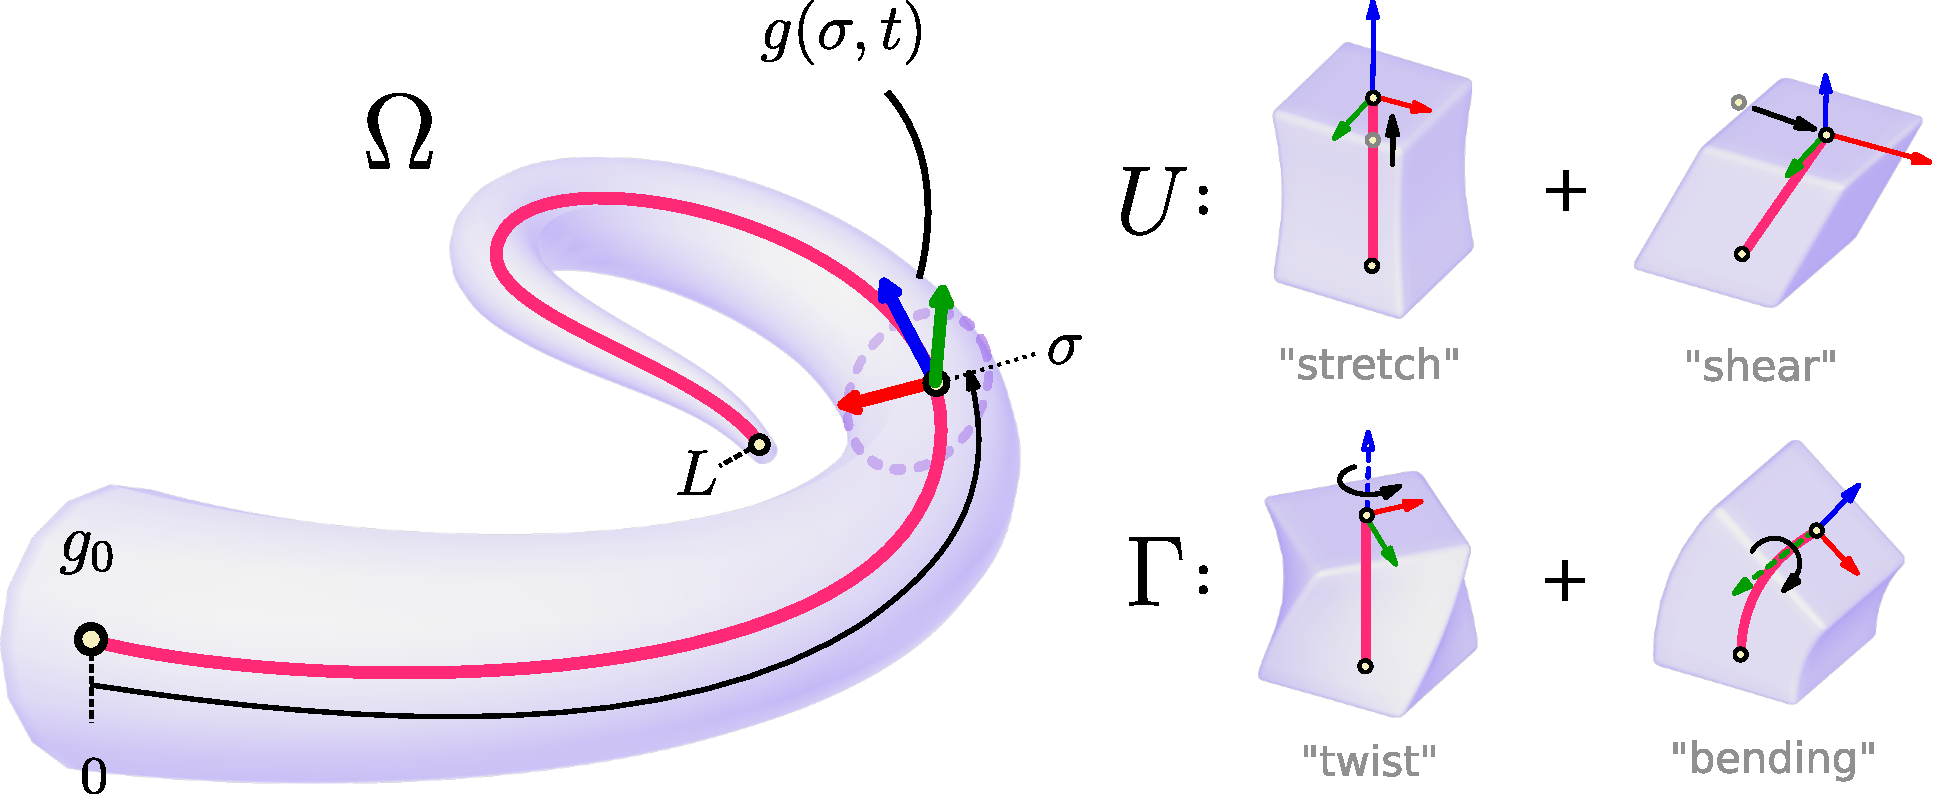
\includegraphics[width=0.85\textwidth]{./pdf/thesis-figure-cosserat.pdf}
\caption{Illustration of the soft beam model using geometric Cosserat beam theory, where the backbone curve is $\gB(\sigma,t) \in \mathrm{SE}(3)$ shown as \data{magenta}. The geometric strain vector $\xiB := \textrm{vec}\left\{ \GammaB, \UB\right\}$ a vector of size 6 consisting of stretch-shear strains $\UB$ and twist-bending strains $\GammaB$.}   
\label{fig:C5:CosseratExample}
\vspace{-3mm}  
\end{figure}

\textbf{A: Computationally-efficient soft beam models.} Following the geometric Cosserat beam frameworks \cite{Renda2020,Boyer2020,Caasenbrood2022Nov}, the reduced nonlinear dynamics of a soft beam model, fixed to a non-inertial base, can be represented using a Lagrangian formulation:
%
\begin{multline}
\MB(\q)\ddq + \CB(\q,\dq)\dq + \fB_{\textrm{mat}}(\q,\dq) + \fB\grav(\q) =  \fB_{\Omega_{\textrm{env}}} (\q,\dq) + \tauB(\q,\uB),
\label{eq:C5:model_beam}
\end{multline}
%
where $\q$, $\dq$, and $\ddq$ represent the modal coefficients, velocity, and acceleration, respectively; $\MB$ denotes a state-dependent generalized inertia matrix, and $\CB$ denotes the Coriolis matrix. The material forces are expressed as $\fB_{\textrm{mat}}(\q,\dq) = \KB(\q) \q + \RB \dq$, where $\KB$ is a generalized stiffness matrix and $\RB$ is a generalized damping matrix. The environmental forces are represented by the vector $\fB_{\Omega_{\textrm{env}}}$, and the generalized input is given by $\tauB := \GB \uB$, where $\GB(\q)$ is the input mapping. As in Section \ref{sec:C5:fem}, material and contact models can be assigned using comparable syntax, \code{Shapes.addMaterial} and \code{Shapes.addContact}, respectively. The intrinsic length of a curve can be altered by utilizing the function \code{Shapes.setLength}, while its cross-sectional geometry can be modified through the function \code{Shapes.setGeometry(sdf)}, which accepts a two-dimenional SDF function that may be arbitrarily complex.

Due to the complexity of deriving the forward kinematics and dynamics in the Cosserat model, the following subsections provide a clear summary of the finite-dimensional basis representation and its relationship to reduced kinematics. The system matrices, on the other hand, are notoriously lengthy expressions and thus omitted in this work. The reader is referred to \cite{Caasenbrood2022Nov} for a full derivation of model \eqref{eq:C5:model_beam}.

\textbf{B: Finite dimensional projection.} To start, our aim is to obtain a finite-dimensional approximation of the local geometric strain vector, denoted as $\xiB:= (\gB\inv \tfrac{\p \gB}{\p \sigma})^\wedge := (\GammaB^\top,\,\UB^\top)^\top$, where $\sigma \in [0,L]$ is a spatial coordinate and $(\cdot)^{\wedge}: \textrm{se}(3) \to \R^6$ (see \cite{Murray2017Sep}). Here, $\Gamma_{i}$ and $U_{i}$ are the torsion-curvature and elongation-shear curve parameters, respectively. To achieve this, we employ a Ritz-Galerkin modal discretization approach following the work of Boyer et al. \cite{Boyer2020}. This approach assumes that the strain can be accurately represented through a finite series of orthonormal basis functions:
%
\begin{align}
[\xi_i]_{\thetaB_i}(\sigma,\q_i) & = \sum_{j=1}^{k_i} \theta_{i,j}(\sigma) q_{i,j} + \xi_i^\circ (\sigma), \notag \\ & = \underbrace{\big[\theta_{i,1}(\sigma)\; \hdots\; \theta_{i,k_i} (\sigma) \big]}_{\thetaB_i^\top(\sigma)} \q_i + \xi_i^\circ(\sigma)
\end{align}
%
where $\thetaB_i$ is the modal approximation vector related to the $i$-th strain component, $\q_i$ is its corresponding modal coefficient, and $[\cdot]_{\thetaB}$ denotes the subspace projection operator. By collecting all terms $q_{i,j}$ and $\theta_{i,j}$, we compactly express the finite-dimensional approximation as an affine operation:
%
\begin{equation}
[\xiB]_{\ThetaB}(\sigma,\q) = \ThetaB^{\!\top}\!(\sigma) \q + \xiB^{\circ}(\sigma)
\label{eq:C5:xi_computation_POD}
\end{equation}
%
where $\ThetaB:= \textrm{blkdiag}\{\thetaB_1,\dots,\thetaB_6\}$ is referred to as the \textit{"modal approximation matrix"}, and $\q:=\textrm{vec}\{\q_1,\dots,\q_6\}$ is the generalized coordinate vector of the global soft beam model in \eqref{eq:C5:model_beam}. Note that a geometric strain entry may be constrained and therefore not contribute to the overall continuum dynamics, thus $\thetaB_i,\q_i \in \emptyset$ without loss of generality. The choice of basis plays a crucial role and often relies on \textit{ad-hoc} approaches. It is therefore critical to choose an appropriate basis for optimal performance of the soft robot model.
% 
\begin{figure}[!t]
\centering
\includegraphics*[width=0.5\textwidth]{./pdf/thesis-figure-6-11.pdf}
%\input{./fig/fig_shp_basisspace.tex}
\caption{The library of modal basis functions is implemented in the Sorotoki toolkit, with a modal ordering of \{\ldata{Matlab1}, \ldata{Matlab2}, \ldata{Matlab3}\}. These function bases include Piecewise Constant Curvature (PCC), Piecewise Linear (PWL), full and piecewise Chebyshev, and full and piecewise Bernstein polynomials.}
\label{fig:C5:shapesexample}
\vspace{-5mm}
\end{figure}

\textbf{C: Library of modal strain bases.} In \textit{Sorotoki}, the general constructor for creating a modal basis is defined as \code{pod = Basis(N,M,'type')}, where \code{N} represents the number of samples (i.e., the level of discretization of the spatial curve), \code{M} is the degree of the basis, and \code{'type'} is a character input that specifies the basis type.

The literature presents various types of modal bases, with the Piecewise Constant Curvature (PCC) approach being the most commonly used \cite{Falkenhahn2015May,DellaSantina2021Oct}. The Piecewise Constant Curvature approach is suitable for certain conditions, for example, when homogeneous bending moment and homogeneous material properties are considered. However, it lacks the ability to ensure the continuity of the strain field at the boundaries between sections, resulting in jumps in the strain profile. As a result, researchers have been exploring alternative representations that more effectively preserve the continuity conditions of the deformable continuums. Examples of alternative representations of bases include piecewise linear \cite{Li2023Jan}, affine curvature \cite{Santina2020Dec,Stella2022Nov}, Fourier cosine/sine series \cite{Chirikjian2015Jul,Chirikjian1994Jun}, Legendre or Chebyshev \cite{Boyer2020,Caasenbrood2022Nov}, and actuation load bases \cite{Renda2020Apr}. The \textit{Sorotoki} package offers access to a library of anonymous functions, facilitating the utilization of a range of basis functions. As an illustration, a collection of basis functions is displayed in Figure \ref{fig:C5:shapesexample}.\\

\begin{rmk}[On the modal order]
Generally, finding a suitable reduction basis and reduction order can be a challenging task. The general assumption is that if the basis belongs to a regular function space (\ie, Sobolev space) and the modal index $k_i$ goes to infinity, the strain approximation converges (uniformly) to the exact solution on the interval $[0,L]$. However, as increasing the modal order enhances precision, it also greatly impacts computational performance. Thus, finding a balance between accuracy and computational speed is of utmost importance for the successful implementation of soft robotic models, often requiring an \textit{ad-hoc} approach.
\end{rmk}


\label{sec:C5:femPODbasis}
\textbf{C: Data-driven strain basis from offline FEM simulations.} To address the challenges of improving efficacy in the modal reduction of soft beam models, we propose a novel approach that merges the finite element method and soft beam modeling. This approach involves extracting geometric modal information from FEM simulation data to construct a low-dimensional strain basis, which we refer to as the Data-driven Variable Strain (DVS) basis. The DVS basis is similar in concept to the snapshot method presented by the SOFA toolkit \cite{Duriez2016,Coevoet2017,Goury2018}, but adapted for use with one-dimensional curves. It takes into account the underlying geometric features of the soft robot and represents them in a minimal subspace representation. This approach leads to a substantial reduction in the number of states while still maintaining high accuracy in deformations, high computational efficiency, and providing a clear structure for passive and active joints. The derivation has two steps: \\

\textbf{Step 1: Recovery of geometric strain from FEM:} The reconstruction of the MIVS basis begins with obtaining geometric strain data from a Finite Element Method (FEM) simulation. The simulation is carried out using either \code{Fem.simulate} or \code{Fem.solve}, and the resultant information is stored in the \code{fem.Log} data structure. Mathematically, the simulation retrieves the states $\xB^{(i)}:=\xB(t_i)$ at discrete time instances $t_i \in \{0,...,T\}$, which in turn provides us with nodal position vectors $\pB$ and the deformation gradient $\FB$ at any point in the mesh. Using the polar decomposition $\QB = \FB\VB \inv \in \textrm{SO}(3)$, see Table \ref{tab:C5:strain_measures}, we can retrieve the rigid body transformation of the FEM mesh
%
$$\gB_{\textrm{FEM}}(\sB, \x^{(i)}) = \begin{pmatrix} \QB(\sB,\x^{(i)}) & \pB(\sB,\x^{(i)}) \\ \vec{0} & 1 \end{pmatrix},$$
%
where $\sB \subseteq \Omega$ is a spatial location within the undeformed mesh. It is important to note that if $\sB$ does not correspond to a nodal location of the mesh, interpolation using elemental shape functions is necessary. Now, let $\bar{\gammaB}: [0,L] \to \Omega$ be a unit-speed reference backbone curve that is contained within the mesh domain $\Omega$. Then, we can retrieve $\gB_{\textrm{FEM}}(\bar{\gammaB},\x^{(i)})$. Subsequently, the geometric strain can be approximated as $\xiB_{\textrm{FEM}} \approx (\gB_{\textrm{FEM}})\inv \delta \gB_{\textrm{FEM}}$. Here, $\delta \gB_{\textrm{FEM}}$ represents the spatial derivative of the reference curve w.r.t. $\sigma$, which is calculated using the central difference method. It is worth noting that the choice of $\bar{\gammaB}$ is free, allowing for the estimation of geometric strain for many complex structures. The full procedure is outlined in Algorithm \ref{algo:C5:fem_reconstruction}. \\
%
\begin{algorithm}[!t]
    \caption{Recover geometric strain field $\xiB_{\textrm{FEM}}$ from offline FEM simulation data. \label{algo:C5:fem_reconstruction}}
    \KwIn{Nodal displacements $\xB$, mesh tesselation $\mathcal{T}$, reference curve $\bar{\gammaB}$, and sample set $\mathcal{S}$}
    \KwOut{Geometric strain field $\xiB_{\textrm{FEM}}$ at time $t_i$ \label{algo:C5:strainFEM}}
    
    %\tcp{assemble SE(3) from Mesh}

    %backbone curve $\mathcal{C} \gets \texttt{ForwardKinematics}(\mathcal{S})$\;

    \For{$i$ = each spatial sample $\sigma_i \in \mathcal{S}$}
    {
        get reference position $\bar{\pB} \gets \bar{\gammaB}(\sigma_i)$ \;
        get element $\mathcal{E} \gets \texttt{inElement}(\bar{\pB},\mathcal{T})$ \;
        \If{$\mathcal{E} == \emptyset$}
        {
            get edge $\mathcal{E} \gets \texttt{onClosestEdge}(\bar{\pB},\mathcal{T})$\;
        }
        initialize $\mat{\Phi}^{(0)} \gets \mat{I}_3$ \;
        initialize $\delta \gammaB^{(0)} \gets \vec{0}_3$ \;
        \For{$j = $ each vertex spanned by element $\mathcal{E}$}
        {
            get nodal displacement $\vec{X} \gets \texttt{FEM}(\mat{x}_j)$ \;
            get deformation gradient $\mat{Y} \gets \texttt{FEM}(\mat{x}_j)$ \;
            $[\mat{Q},\,\mat{V}] \gets \texttt{PolarDecomposition}(\mat{Y})$ \;
            $\alpha \gets \texttt{ElementInterpolation}(\bar{\pB})$ \;
            update $\PhiB^{(j)} \gets \texttt{AverageSO3}(\PhiB^{(j)},\alpha\mat{Q})$ \;
            update $\delta\gammaB^{(j)} \gets \delta\gammaB^{(j)} + \alpha \vec{X}$ \;
        }
        $\gB_{\textrm{FEM}}^{(i)} \gets \texttt{SE3}(\PhiB^{(j)},\bar{\pB} + \delta\gammaB^{(j)})$\;
    }

    \For{$i$ = each spatial sample $\sigma_i \in \mathcal{S}$}{
    $\delta\gB_{\textrm{FEM}}^{(i)} \gets \texttt{CentralDiff}(\gB_{\textrm{FEM}}^{(i-1)},\gB_{\textrm{FEM}}^{(i+1)})$ \;
    assemble strain $\vec{\xi}_{\textrm{FEM}}^{(i)} \gets (\gB_{\textrm{FEM}}^{(i)})\inv \delta\gB_{\textrm{FEM}}^{(i)}$\;
    }
\end{algorithm}

\textbf{Step 2: POD snapshot basis:} Next, we employ the "Snapshot Proper Orthogonal Decomposition" (POD) as described in \cite{Duriez2016,Goury2018}. This data-driven approach determines a suitable orthonormal basis from simulated or experimental data \cite{Astrid2008}. Let $y_{i}(\sigma,t) := \xi_{\textrm{FEM},i}(\sigma,t)$ represent the measurement of the $i$-th entry of the strain $\xiB_{\textrm{FEM}}$. For each discrete time $t_i$, the sample is condensed into a column vector $\vec{y}_i^{(t)} := \textrm{col}\left\{y_i(0,t),\dots,y_i(L,t) \right\}$ and then stacked into the "snapshot matrix" $\mat{S}_i = \textrm{row}\left\{ \vec{y}_i^{(0)},\dots,\vec{y}_i^{(T)} \right\}$ where $T$ is the finite horizon time. The correlation matrix $\mat{\mathcal{C}}_i = \tfrac{1}{m} \mat{S}_i^\top \mat{S}_i$ is then computed with $m = \dim(\yB_i)$, and the spectral decomposition is performed:
%
\begin{equation}
\mat{\mathcal{C}}_i \VB_i = \mat{\lambda}_i \VB_i,
\end{equation}
%
where $\VB_i = \textrm{row}\{\vB_{i,1},,...\vB_{i,m}\}$ is a basis of eigenvectors and $\mat{\lambda}_i = \diag{\lambda_{i,1},,...,\lambda_{i,m}}$ is a diagonal matrix of sorted eigenvalues. By selecting $k_i \le m$ such that $\lambda_{i,k_i} \le \delta$, where $\delta$ is a desired threshold, we obtain a truncated orthonormal basis $\{\vB_{i,j}\}_{j=1}^{k_i}$. This process is repeated until the modal interpolation matrix $\ThetaB$, required for \eqref{eq:C5:xi_computation_POD}, is fully obtained. Finally, a Gram–Schmidt orthogonalization procedure is performed to ensure that its columns are mutually orthogonal. \\

\begin{figure}[!t]
\centering
\includegraphics*[width=.815\textwidth]{./pdf/thesis-figure-6-11-2.pdf}  \\[0.15em]
\includegraphics*[width=.815\textwidth]{./pdf/thesis-figure-6-11-3.pdf}% \\[1.15em]
%\includegraphics*[width=.85\textwidth]{./pdf/thesis-figure-6-11-1.pdf} \\[0.15em]
%\input{./fig/fig_GVISmode_fem.tex} \\[0.75em]
%\input{./fig/fig_GVISmode.tex} \\[0.21em]
%\input{./fig/fig_GVISmode_pos.tex} 
\caption{Example reconstruction of the Data-driven Variable Strain (DVS) basis for a PneuNet actuator grasping a cylindrical object. (top) The first three modes of the DVS basis related to planar bending, \ie., planar curvature. The ordering is $\{$\ldata{Matlab1}, \ldata{Matlab2}, \ldata{Matlab3}$\}$. (bottom) A comparison between the true physical system, the FEM model, and the soft beam model shown in \data{magenta}.}
%\vspace{-3mm}
\label{fig:C5:gvis_modes}
\end{figure}
%

\begin{figure}[!t]
\centering
\includegraphics*[width=.85\textwidth]{./pdf/thesis-figure-6-11-1.pdf} \\[0.15em]
%\input{./fig/fig_GVISmode_fem.tex} \\[0.75em]
%\input{./fig/fig_GVISmode.tex} \\[0.21em]
%\input{./fig/fig_GVISmode_pos.tex} 
\caption{Example reconstruction of the Data-driven Variable Strain (DVS) basis for a PneuNet actuator grasping a cylindrical object. A comparison between the true physical system, the FEM model, and the soft beam model shown in \data{magenta}.}
\vspace{-3mm}
\label{fig:C5:gvis_experiment}
\end{figure}

\begin{example}{Data-driven basis from PneuNet simulation}
To demonstrate the reconstruction of the DVS basis, we consider a soft bending actuation, also known as the PneuNet actuator. A FEM simulation model is constructed where the soft actuator is subjected to a linearly increasing pressure up to $40$ \si{\kilo \pascal} and curls around a cylindrical object when pressurized. Figure \ref{fig:C5:gvis_modes} (top) illustrates the true system and the FEM simulation obtained through \code{fem.simulate}. The FEM class is then integrated into the \class{Shapes} class through the syntax \code{shp = Shapes(fem,dof)}, where \code{dof = [0,3,0,0,0,0]} indicates the desire to recover the first three curvature bending modes from the \code{fem} object class. The length and base orientation are specified using \code{shp.setLength} and \code{shp.setBase}, respectively. The basis is then reconstructed by calling \code{shp.reconstruct}. The first three curvature bending modes are displayed in Figure \ref{fig:C5:gvis_modes} (bottom). It can be observed that the geometrical features of the PneuNet actuator are encoded in the basis, with the 12 embedded pressure chambers represented by the DVS strain basis. The associated code is provided below:
\end{example}

\begin{lstlisting}[style=matlab]   
%% EXAMPLE: Shapes class (DVS basis)   
fem = load('femPneuNet.mat');   % load fem model

dof = [0,M,0,0,0,0];  % pure planar curvature bending
shp = Shapes(fem, dof, 'NNode', 200, 'Length',105);

% generate DVS basis 
shp = shp.reference(@(s) [s,0,0].' );
shp = shp.reconstruct();
\end{lstlisting}
%


\textbf{D: Forward beam kinematics.} Once a basis representation $\ThetaB$ has been selected, the forward kinematics of the continuum body can be efficiently solved using exponential maps for the group $\SE{3}$. As such, the backbone curve is be approximated by
%
\begin{equation}
    [\gB]_{\ThetaB}(\sigma,\q) = \gB_0 \exp_{\textrm{SE}(3)} \left[ \int_0^\sigma {[\hat{\xiB}]_\ThetaB}(s,\q) \; ds\right]
    \label{eq:C5:gcurve}
\end{equation}
%
On the other hand, the local velocity twist is represented by $\etaB:= (\gB\inv\dot{\gB})^{\vee}$, which, similarly to rigid robotics, is linear in the joint velocities $\dot{\q}$. Regarding computation, the velocity twist of a point $\sigma$ on the curve $\gB$ can be represented as follows:
%
\begin{align}
    [\etaB]_\ThetaB(\sigma,\cdot) & = \left[\mat{Ad}^{-1}_{[\gB](\sigma,\q)}\int_{0}^\sigma  \mat{Ad}_{[\gB](s,\q)} \ThetaB(s)\; ds \right]  \dq,  \notag \\
                                  & =: \JB(\sigma,\q) \dq,
                                  \label{eq:C5:eta}                                  
\end{align}
%
where $\JB(\sigma,\q)$ denotes the geometric Jacobian that maps the joint velocities $\dq$ to velocity twist. For concisness, we write $\JB_\sigma := \JB(\sigma,\cdot)$. The Jacobian matrix holds significance not only for inverse kinematics but also for mapping external wrenches onto the generalized joint torques. For instance, it can be used to calculate the environmental forces as $\fB_{\Omega_{\textrm{env}}} = \int_0^L \JB_\sigma^\top \FT_{\textrm{env}} \; d\sigma$, where $\FT_{\textrm{env}}$ represents a wrench related to the environment $\Omega_{\textrm{env}}$ described by SDFs. 

Given the expressions in \eqref{eq:C5:xi_computation_POD}, \eqref{eq:C5:gcurve}, and \eqref{eq:C5:eta}, we can numerically evaluate the forward kinematics. We use a two-step Runge-Kutta integration solver that approximates the spatial integration. The forward kinematics solver is called by \code{shp = Shapes.string(q,dq)}, which stores all necessary numerical evaluations into a data structure \code{shp.Log.FK}. To further improve computation speed, \code{.mex} executable files are utilized.


\textbf{E: Inverse beam kinematics (shape control).} \label{sec:C5:inverseKinematics} The inverse kinematics problem for soft continuum manipulators involves finding a solution $\q$ such that either ($i$) the end-effector reaches a specified setpoint, or ($ii$) shape control of the backbone is achieved. These manipulators often exhibit high levels of redundancy, so called hyper-redundancy \cite{Chirikjian1994Jun}; leading to different solution approaches common to rigid robotics. Few modal basis representations possess a closed-form solution to the inverse kinematics, and they are typically solved using an iterative numerical method (\eg, Newton Raphson). In \textit{Sorotoki}, the inverse kinematics solver for sof beam models is implemented  as \code{Shapes.IK}. We briefly detail the theory.

Suppose the desired shape of the soft manipulator is $\gB^\star(\sigma) \in \WT_\sigma$ with 
%
\begin{equation}
\WT_\sigma := \big\{ \XB \in \mathrm{SE}(3)\;|\; \XB = [\gB]_\ThetaB(\sigma,\q),\, \q \in \mathcal{Q} \big\}    
\end{equation}
%
the set of possible configurations of the backbone curve at $\sigma$. Note that $\WT_L$ spans the workspace of the end-effector, and $\WT_\Omega := \{\WT_\sigma \;|\; \sigma \in [0,L]\}$ the workspace of the entire soft body. For sake of readability, we redefine $\gB_i(\q) := [\gB]_\ThetaB(\sigma_i,\q)$ and $\gB^\star_{i} := \gB^\star(\sigma_i)$. We also redefine the geometric Jacobian by $\JB_i(\q) := \JB(\sigma_i,\q)$.

Then, the inverse shape kinematics problem for the discretized soft manipulator can be formualted as an optimization problem of the form:
%
\begin{mini}[2]
    {\q}{\Phi = \sum_{i=1}^{N_p}  \Big\lVert \KB_p\textrm{Log}_{\textrm{SE}(3)}\left[ \gB_i\inv(\q)\gB^\star_{i}\right]^{\vee} \Big \rVert_2}{}{}
    \addConstraint{\gB_i, \gB^\star_i\in \mathcal{W}_{\Omega},}{}{}
\end{mini}
%
where $\textrm{Log}_{\textrm{SE}(3)}$ denotes the logarithmic mapping from the Lie group to its algebra, see \cite{Murray2017Sep}. Despite the highly nonlinear nature of the optimization problem, its solution procedure is relatively straightforward two-step procedure:

Given an initial guess $\q^{(0)} \in \mathcal{Q}$, the aim is to compute an incremental update step that brings us closer to a local minimizer of the objective function $\Phi$. For clarity, let $\vec{\Xi}_i :=\gB\inv_i\gB^\star_i$ represent the geometric error between the soft robot and the desired shape. The state increment can then be expressed as:
%
\begin{align}
\vec{\lambda}_i^{(k)} & = \JB_i^\top (\q^{(k)}) \left[ \KB_{p} \textrm{T}_{\textrm{SE}(3)}(\vec{\Xi}_i) \textrm{Log}_{\textrm{SE}(3)} (\vec{\Xi}_i) \right]^\vee, \label{eq:C5:invkin1}\\
\q^{(k+1)} & = \q^{(k)} + \sum^{N_p}_{i = 1} \vec{\Lambda}_i \left[\vec{\lambda}^{(k)}  - \NT_i(\q^{(k)}) \nabla \Phi_{\textrm{sub}} \right],
\label{eq:C5:invkin2}
\end{align}
%
where $\textrm{T}_{\textrm{SE}(3)}$ denotes the tangent operator map on the group $\mathrm{SE}(3)$, see \cite{Bullo1995}, $\KB_p$ an artifical stiffness tensor, $\NT_i = (\IB - \JB_{i}\JB_{i}^\top)$ represents the null-space projection, and $\vec{\Lambda}_i$ a diagonal activation matrix. The trivial choice is $\LambdaB_i = \IB_n$. The nullspace projector can be extremely useful in exploring the high redundancy in soft robots, allows us to consider subtasks described by $\Phi_\textrm{sub}$. Classical examples of such subtasks include: minimizing elastic energy or obstacle avoidance. The iterative solver in \eqref{eq:C5:invkin1} and \eqref{eq:C5:invkin2} until convergence is $\q^{(k)}$ is achieved. \\

\begin{example}[Contact kinematics of ultra-gentle soft gripper]
To showcase the forward and inverse kinematic solvers of Sorotoki, we will describe the ultra-gentle underwater soft gripper developed by Sinatra et al. \cite{Sinatra2019Aug}. The soft gripper consists of six soft fingers attached to a rigid palm base, where each soft gripper was designed to apply low contact pressure and minimize harm to common jellyfish species. An illustration of the sysem is shown in Figure \ref{fig:C5:shapesexample}. The delicate compliance of the soft gripper is achieved through the use of an extremely low durometer silicone matrix (Shore 20A). The actuator has a simple rectangular geometry, with a narrow cross-section of approximately 10 $\times$ 2 \si{\milli \meter} and an internal off-center rectangular hole. The thinnest part of the soft actuator, called the membrane, is approximately 0.35 \si{\milli \meter} thick, and length of about 130 \si{\milli \meter}.

In this study, we aim to reproduce a grasping scenario of a jellyfish modeled as a static SDF object. To achieve this, we first initiate a soft finger by utilizing the \class{Shapes} class. We employ a third-order Chebyshev basis to approximate the strain field. The geometric properties of the soft finger are specified through the functions \code{Shapes.setLength} and \code{Shapes.setGeometry}. Using a for-loop, we generate each soft finger sequentially, defining the spatial location of the fixed base with \code{Shapes.setBase}. Prior to deployment, each soft finger undergoes predeformation, which is calculated through the application of the forward kinematics solver \code{Shapes.FK(q)}. The joint configuration, \code{q}, is selected to match the experiments presented in Figure \ref{fig:C5:shapesexample}.

Subsequently, the deformed backbone is projected onto the surface of the SDF jellyfish through the use of the function \code{sdf.project}. The inverse kinematics solver is then invoked with \code{Shapes.IK}, resulting in the image depicted in Figure \ref{fig:C5:shapesexample}. Note that the inverse kinematics solver effectively places the soft finger onto the surface of the SDF object without causing penetration. The code for the forward and inverse kinematics is presented below:
\end{example}
\vfill
\begin{figure}[!t]
\centering
\includegraphics*[width=.95\textwidth]{./pdf/thesis-figure-6-13.pdf}
%\input{./fig/fig_mdl_example2.tex} \\[0.01em]
%\input{./fig/fig_mdl_example2_grasp.tex}
%\vspace{-5mm}
\caption{(Top) A snapshot of the ultra-gentle soft robot gripper developed by Sinatra et al. \cite{Sinatra2019Aug} is shown, demonstrating its ability to grasp a delicate jellyfish. (Bottom) The reconstructed soft gripper using \textit{Sorotoki} is presented, where each tentacle finger is modeled individually using the \textit{Shapes} class. It can be observed that the soft tentacles envelop the SDF object without penetration, indicating the successful accomplishment of task and subtask.}
\label{fig:C5:shapesexample}
\vspace{-5mm}
\end{figure}

\begin{lstlisting}[style=matlab] 
%% EXAMPLE: Shapes class (for/inv kinematics) 
sdf = sSphere(0,0,-60,40)   % jellyfish SDF

% -- generate Shapes class 
N = 200;                      % discretization
M = 3;                        % number of modes
pod = Basis(N,M,'chebyshev'); % build orth. basis
dof = [0,M,M,0,0,0];          % geom. strain dof

shp = Shapes(pod,dof,'Length',120);
shp = shp.setGeometry(sRectangle(4,1));

% -- inverse kinematics on SDF topology 
for k = 1:6
    shp = shp.setBase(G{k});  % set base SE(3)

    pos = shp.FK(q0{k});    % forward kin.
    prj = sdf.project(pos); % project points

    qd  = shp.IK(prj);      % inverse kin.
    shp.render(qd);         % render shape
end

sdf.show();  % render jellyfish
\end{lstlisting}